\scanpage{15}
\figure{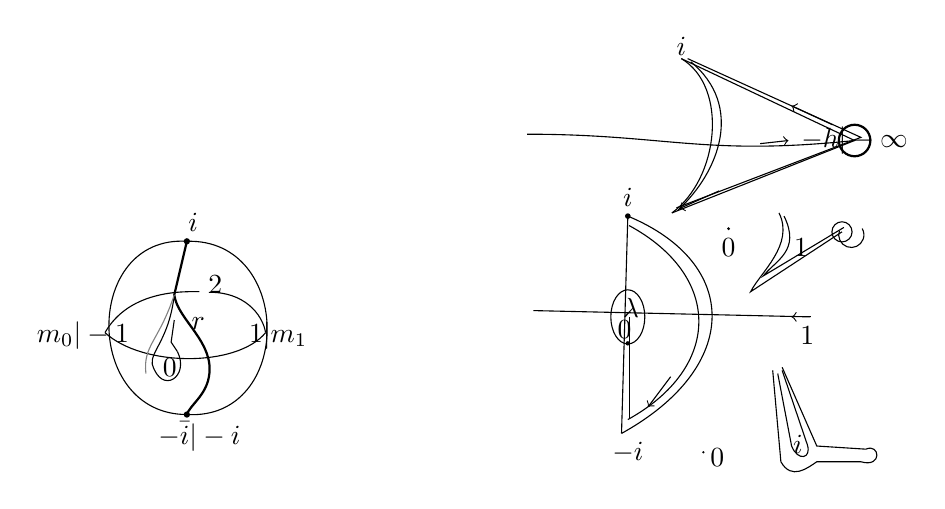
\begin{tikzpicture}[x=.8cm,y=.8cm]
\draw (1.8,3.65)..controls(.15,3.75)and(.15,.9)..(1.8,.9)..controls(3.5,.8)and(3.5,3.7)..(1.8,3.65);
\draw (.5,2.2)..controls(1.1,1.65)and(2.6,1.65)..(3.05,2.2);
\draw (.5,2.2)..controls(.9,2.9)and(1.8,2.85)..(2.0,2.85);
\draw (2.15,2.84)..controls(2.7,2.85)and(3,2.5)..(3.05,2.2);
\draw[thick] (1.8,3.65)--(1.6,2.8)..controls(1.65,2.4)and(2.25,2.05)..(2.15,1.5)..controls(2.1,1.2)and(1.85,1.05)..(1.8,.9);
\draw (1.6,2.8)..controls(1.52,2.1)and(1.22,1.9)..(1.25,1.7)..controls(1.4,1.2)and(1.85,1.5)..(1.65,1.9);
\draw (1.6,2.4)--(1.55,2.05)--(1.65,1.9);
\draw[gray] (1.6,2.8)..controls(1.35,2.05)and(1.1,2)..(1.15,1.55);
\fill (1.8,3.65) circle(.05);\fill (1.8,.9) circle(.05);
\node at (1.9,3.95) {$i$};\node at (2,.55) {$\unsure{-\bar i|-i}$};
\node at (.15,2.15) {$\unsure{m_0|-1}$};\node at (3.25,2.15) {$\unsure{1|m_1}$};
\node at (2.25,2.96) {$2$};\node at (1.53,1.65) {$0$};\node at (1.98,2.35) {$\unsure{r}$};
\draw (9.65,6.55)--(12.4,5.25)--(9.5,4.1);
\draw (9.75,6.55)--(12.5,5.3)--(9.57,4.18);
\draw (9.65,6.55)..controls(10.4,6.1)and(10.25,4.65)..(9.5,4.1);
\draw (9.8,6.5)..controls(10.65,5.8)and(10.25,4.75)..(9.6,4.15);
\draw[->] (12.05,5.5)--(11.4,5.8);\draw[->] (10.25,4.45)--(9.62,4.17);
\draw (7.2,5.35)..controls(9.4,5.35)and(10,5)..(12.4,5.25);
\draw[->] (10.9,5.2)--(11.35,5.25);
\draw[thick] (12.4,5.25) circle(.25);\node at (12.4,5.25) {$\unsure{-h|-\infty}$};
\node at (9.65,6.75) {$\unsure{i}$};
\draw (8.8,4.05)--(8.7,.6);
\draw (8.8,4.05)..controls(10.6,3.3)and(10.6,1.65)..(8.7,.6);
\draw (8.82,3.9)..controls(10.3,3.1)and(10.3,1.65)..(8.8,.82);
\draw (8.82,2.45)--(8.82,.85);\draw[->] (9.48,1.5)--(9.12,1.02);
\draw (7.3,2.55)--(11.7,2.45);\draw[->] (11.7,2.45)--(11.4,2.45);
\draw (8.8,2.45) ellipse (.27 and .43);
\node at (8.85,2.6) {$\unsure{\lambda}$};\node at (8.75,2.25) {$0$};
\node at (8.8,4.35) {$i$};\node at (8.8,.3) {$-i$};\node at (11.65,2.15) {$1$};
\fill (8.8,4.05) circle(.045);\fill (8.8,2.03) circle(.035);
\node at (10.4,3.55) {$0$};\fill (10.4,3.85) circle(.025);
\draw (11.2,4.1)..controls(11.45,3.6)and(10.9,3.15)..(10.75,2.85)--(12.2,3.8);
\draw (11.28,4.05)..controls(11.55,3.5)and(11.15,3.35)..(10.95,3.1)--(12.23,3.87);
\draw (12.2,3.8) circle(.16);\draw (12.16,3.82) arc[start angle=160,end angle=390,radius=.2];
\node at (11.55,3.55) {$\unsure{1}$};
\draw (11.1,1.6)--(11.23,.15)..controls(11.4,-.15)and(11.65,.05)..(11.8,.15)--(12.5,.15)..controls(12.85,.05)and(12.8,.45)..(12.58,.35)--(11.8,.4)--(11.25,1.65);
\draw (11.18,1.55)--(11.4,.4)..controls(11.5,.15)and(11.72,.2)..(11.65,.42)--(11.25,1.6);
\node at (11.5,.42) {$\unsure{i}$};
\fill (10,.3) circle(.02);\node at (10.22,.21) {$0$};
\end{tikzpicture}}

\[
\pi\qquad\lambda_0\ \lambda_1\ \lambda_2\ \lambda_3\qquad\varepsilon
\]
\deleted{\[
\lambda_0\lambda_1\lambda_2\lambda_3=1
\]}
\deleted{\[
\lambda_3\lambda_2\lambda_1\lambda_0=1
\]}
\[
\varepsilon^2=1\qquad
\begin{cases}\varepsilon\lambda_0\varepsilon^{-1}=\lambda_0^{-1}\\
\varepsilon\lambda_1\varepsilon^{-1}=\lambda_{\unsure{1}}^{-1}
\end{cases}
\qquad\varepsilon\lambda_i\varepsilon^{-1}
\]
\[
\operatorname{Hom}(i,-i)
\]
\diagram{\begin{tikzcd}[ampersand replacement=\&,column sep=large,row sep=small]
\operatorname{Hom}(-i,-i)\arrow[d,phantom,"\wr"]\&\operatorname{Hom}(i,i)\arrow[d,phantom,"\wr"]\\
\pi\&\pi
\end{tikzcd}}
\[
\ell\circ\bar\ell\qquad\lambda_1^{-1}\lambda_2^{-1}\lambda_1
\]
\diagram{\begin{tikzcd}[ampersand replacement=\&,column sep=large]
i\arrow[r,"\varepsilon^{-1}"]\&\unsure{\bar i|-i}\&\unsure{\bar i|-i}\arrow[r,"\overset{\longleftarrow}{\lambda_i}"]\&\unsure{\bar i|-i}\&\unsure{\bar i|-i}\arrow[r,"\varepsilon"]\&i
\end{tikzcd}}
\[
\varepsilon\circ\bar\lambda_i\circ\varepsilon^{-1}.
\]

\figure{\begin{tikzpicture}\fill (0,0) circle(.025);\end{tikzpicture}}
\diagram{\begin{tikzcd}[ampersand replacement=\&,row sep=small]
X\arrow[d]\&\Gamma\\\unsure{a}\&
\end{tikzcd}}
\[
(\gamma\in\Gamma,\ell\in\operatorname{Hom}(\gamma a,\deleted{\unsure{\gamma}}b))
\]
\[
(\gamma'\in\Gamma,\ell'\in\operatorname{Hom}(\gamma'b,\deleted{\unsure{\gamma'}}c))
\]
\[
\pi_1(X,\Gamma;a)\mathbin{-}\Gamma
\]

\diagram{\begin{tikzcd}[ampersand replacement=\&,column sep=large,row sep=large]
\gamma a\arrow[r,"\ell"]\&\deleted{\unsure{\gamma}}b\&\deleted{\unsure{\gamma'a\ \gamma'\ell}}:\\
\&\gamma'b\arrow[r,"\ell'"]\&\deleted{\unsure{\gamma'}}c
\end{tikzcd}}
\deleted{\diagram{\begin{tikzcd}[ampersand replacement=\&,column sep=large]
\unsure{\gamma b}\arrow[r,"\unsure{\gamma\ell'}"]\&\unsure{\gamma\gamma'c}
\end{tikzcd}}}

\diagram{\begin{tikzcd}[ampersand replacement=\&,column sep=large]
\gamma'\gamma a\arrow[r,"\gamma'(\ell)"]\&\gamma'b\arrow[r,"\ell'"]\&c
\end{tikzcd}}

\diagram{\begin{tikzcd}[ampersand replacement=\&,column sep=large]
a\arrow[r,dash,"(\gamma\ell')\circ\ell"]\&\gamma\gamma'c
\end{tikzcd}}
\[
(\gamma\gamma',(\gamma\ell')\circ\ell)
\]

\figure{\begin{tikzpicture}
\draw (0,.5)--(-.12,-2.8);
\node at (.7,.2) {$\gamma a$};\fill (1.75,.2) circle(.03);
\node at (.7,-.6) {$-\gamma'a$};\draw (1.35,-.6)--(1.8,-.6);\fill (2.05,-.6) circle(.03);
\end{tikzpicture}}

\[
(\gamma',\ell')\bigl(\gamma^{\deleted{\unsure{\prime}}},\ell^{\deleted{\unsure{\prime}}}\bigr)
=\Bigl(\gamma'\gamma^{\deleted{\unsure{\prime}}},
\deleted{(\unsure{\gamma}\ell')\circ\ell}\inserted{\ell'\circ\gamma'(\ell)}\Bigr)
\]
\figure{\begin{tikzpicture}\draw[thick] (0,0)--(.22,0);\end{tikzpicture}}

\mspage{14}
